% !TeX spellcheck = en_US
\documentclass[a4paper,fontsize=12pt]{scrartcl}
\usepackage{graphicx}
\usepackage{listings}
\usepackage{color}
\usepackage{amsmath}
\usepackage{tikz}
\usepackage{tabularx}

\usetikzlibrary{shapes, arrows, positioning}

\tikzstyle{block} = [draw, rectangle]

\definecolor{mygreen}{rgb}{0,0.6,0}
\definecolor{mygray}{rgb}{0.5,0.5,0.5}
\definecolor{mymauve}{rgb}{0.58,0,0.82}

\lstset{ 
	backgroundcolor=\color{white},   % choose the background color; you must add \usepackage{color} or \usepackage{xcolor}; should come as last argument
	basicstyle=\tiny,        % the size of the fonts that are used for the code
	breakatwhitespace=true,         % sets if automatic breaks should only happen at whitespace
	breaklines=true,                 % sets automatic line breaking
	captionpos=b,                    % sets the caption-position to bottom
	commentstyle=\color{mygreen},    % comment style
	deletekeywords={...},            % if you want to delete keywords from the given language
	escapeinside={\%*}{*)},          % if you want to add LaTeX within your code
	extendedchars=true,              % lets you use non-ASCII characters; for 8-bits encodings only, does not work with UTF-8
	frame=single,	                   % adds a frame around the code
	keepspaces=true,                 % keeps spaces in text, useful for keeping indentation of code (possibly needs columns=flexible)
	keywordstyle=\color{blue},       % keyword style
	language=Octave,                 % the language of the code
	morekeywords={*,...},            % if you want to add more keywords to the set
	numbers=left,                    % where to put the line-numbers; possible values are (none, left, right)
	numbersep=5pt,                   % how far the line-numbers are from the code
	numberstyle=\tiny\color{mygray}, % the style that is used for the line-numbers
	rulecolor=\color{black},         % if not set, the frame-color may be changed on line-breaks within not-black text (e.g. comments (green here))
	showspaces=false,                % show spaces everywhere adding particular underscores; it overrides 'showstringspaces'
	showstringspaces=false,          % underline spaces within strings only
	showtabs=false,                  % show tabs within strings adding particular underscores
	stepnumber=1,                    % the step between two line-numbers. If it's 1, each line will be numbered
	stringstyle=\color{mymauve},     % string literal style
	tabsize=2,	                   % sets default tabsize to 2 spaces
	title=\lstname                   % show the filename of files included with \lstinputlisting; also try caption instead of title
}
\begin{document}
	
	\title{Processor Microarchitecture Exercise Report SoSe 2018}
	\author{Tim Burkert}
	
	\maketitle
	
	\begin{abstract}
		Report, results and evaluation of practical exercises done during processor microarchitecture lecture.
	\end{abstract}
	
	\section{Exercise Description}
	As a practial exercise three different testcases are given. For each testcase four assignments need to be fulfilled.
	
	\paragraph{Testcases}
	
	\begin{description}
		\item Color conversion \\
		RGB color to grayscale with following equation: \\
		$\textbf{intensity} = 0.29894*r + 0.58704*g + 0.11402*b$
		
		\item Histogram calculation \\
		Create a histogram with a given amount of bins for a set of values \\
		$\textbf{histogram[intensity(x,y)]} += 1, \forall (x,y) \in Image$
		
		\item Edge detection \\
		Applying sobel filter to an image \\
		$E(x,y) = I(x,y) * S(x,y)$
	\end{description}
	
	\paragraph{Assigments}
	
	\begin{description}
		\item Write the the program \\
		Experiment in octave \\
		Convert from octave to c \\
		
		\item Analyze classical in-order execution \\
		Compile C to SpartanMC and LEON3 assembly \\
		Analyze the used instructions from the assembly listing a statistics \\
		Profile the execution in ModelSim a statistics \\
		Based on the previous analyses suggest instruction set improvements \\
		
		\item Datapath construction \\
		Construct a statically scheduled pipeline for the computation in C \\
		Get the basic function units from Xilinx Coregen \\
		Verify the datapath in ModelSim against the reference data from C\\
		
		\item Analyze micro-threaded in-order execution \\
		Convert the C program to the SLC language or by hand to the microthreaded assembly. \\
		Profile execution in ModelSim, identify bottlenecks and restructure the program \\
	\end{description}
	
	\section{Color Conversion}
	Conversion form a 24 Bit rgb value to an 8 Bit grayscale value can be done with various precisions and methods. A example using double precision floats is given in octave \textit{rgb2gray}. This method uses a luminosity equation to compute the intensity for each pixel. We implemented the same equation using fixed point arithmetics. For this we firstly converted the luminosities factors for each color to 20 Bit integer value.
	\begin{align*}
		rf &= 0.29894_{10} \approx  0.01001100100001110101_{2} = 313461_{10} * 2^{-20} \\
		gf &= 0.58704_{10} \approx  0.10010110010010000100_{2} = 615556_{10} * 2^{-20} \\
		bf &= 0.11402_{10} \approx  0.00011101001100000111_{2} = 119559_{10} * 2^{-20} \\
	\end{align*}
	To test how different precisions for each factor perform we implemented a following octave function. The function takes an image and a 3x1 vector describing the bit precision for each factor from max 20 to 0. With this function we can test arbitrary bit length combinations.

\begin{lstlisting}
function [J] = ui8rgb2gray (I, bits)
rf = bitshift(uint64(313461), bits(1)-20);  # 0.01001100100001110101
gf = bitshift(uint64(615556), bits(2)-20);  # 0.10010110010010000100
bf = bitshift(uint64(119559), bits(3)-20);  # 0.00011101001100000111
uI = uint64(I);
for i = 1:rows(I)
	for j = 1:columns(I)
		r = rf * uI(i,j,1); g = gf * uI(i,j,2); b = bf * uI(i,j,3);
		J(i,j) = uint8(bitshift(r, -bits(1))) + uint8(bitshift(g, -bits(2))) + uint8(bitshift(b, -bits(3)));
	endfor
endfor
endfunction
\end{lstlisting}

    \subsection{Error Evaluation}

	The total error of rgb to grayscale conversion is a combination of the independent transformation for each channel. The total worst case error is the sum of all three partial worst case errors. Therefore to decide how many bits precision are need for each color channel, we did an error evaluation of each channel. For this we used three different metrics: Maximum Difference, Maximum Weighted Difference and Root Mean Square Error (RMSE)

\paragraph{}
The Maximum Weighted Difference describes the error for a total converted image better then the other metrics. Because the total error of each channel does not effect the total error equal. The total error contribution is depends on the used conversion factors for each channel.
\begin{align*}
 \textbf{intensity} &= 0.29894*r + 0.58704*g + 0.11402*b
\end{align*}


Therefore the green channel twice the error contribution then the red channel and six times the contribution to the blue channel. Because this asymmetric error contribution we chose an asymmetric bit precision for each channel. We used for the green channel 7 Bit precision conversion factor, red channel 6 Bit precision conversion factor and for the blue channel only a 5 Bit precision conversion factor.

\begin{figure}[h]
  \centering
  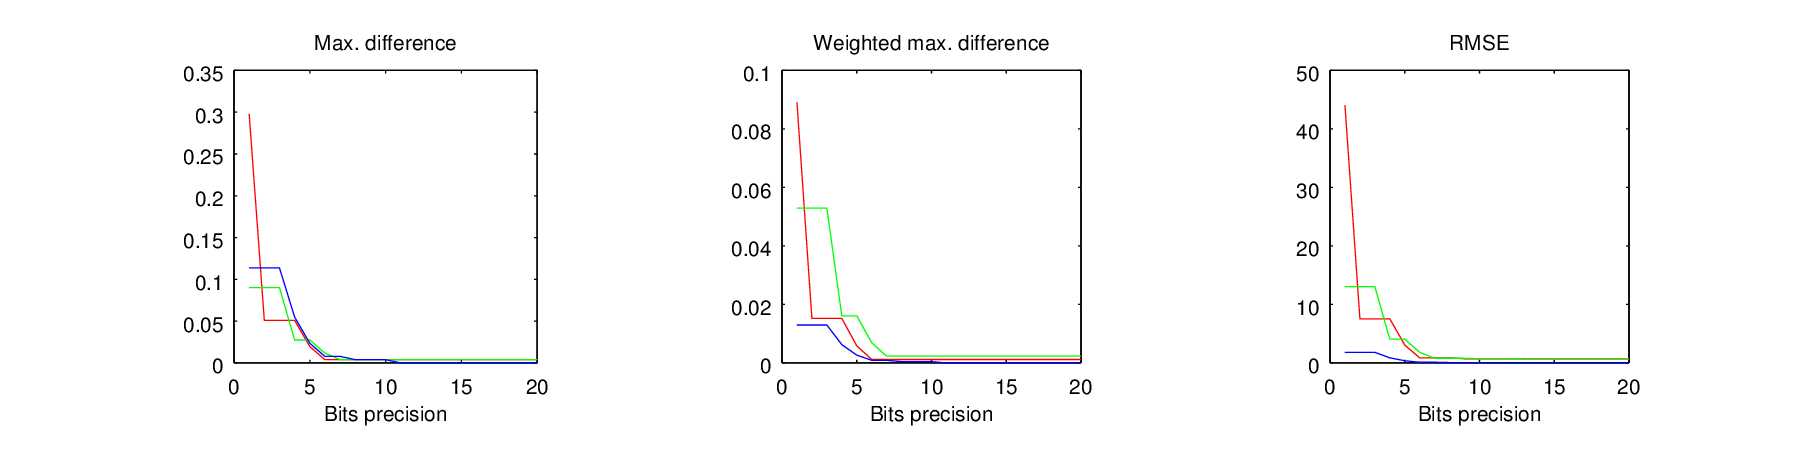
\includegraphics[width=\textwidth]{gray_error} 
  \caption{Maximum difference, weighted maximum difference and RMS Error comparing octave rgb2gray and our implementation.}
\end{figure}


\subsection{C Implementation}

For the c implementation we used a straight forward two dimensional for loop that applies our conversion for each pixel. The rgb2gray function uses the same algorithm as our octave implementation. For validation we exported an small 15x15 image with octave as a constant static input array and printing the resulting array with printf. Therefor we could compare the results for all execution targets. For dynamic code tracing we used following bash script to count which and how many instructions are executed.

\begin{minipage}{\linewidth}

\begin{lstlisting}
grep -n "cpu0" perf-transcript | awk '{print $7}' | sort | uniq -c | sort -hr
\end{lstlisting}
\end{minipage}

\begin{minipage}{\linewidth}
\begin{lstlisting}[language=C]
static inline uint8_t rgb2gray(const uint8_t *p) {
	const uint16_t Rc = 19; //0b0.010011
	const uint16_t Gc = 75; //0b0.1001011
	const uint16_t Bc = 3;  //0b0.00011
	uint8_t nR = (uint8_t)((Rc*p[0])>>6);
	uint8_t nG = (uint8_t)((Gc*p[1])>>7);
	uint8_t nB = (uint8_t)((Bc*p[2])>>5);
	uint8_t res = nR + nG + nB;
	return res;
}
\end{lstlisting}
\end{minipage}

The result of dynamic tracing is attach as a file. Each instruction not executed and therefore not needed can be dropped. This simplifies the processor pipeline, but also restricts the functionality. These kind of optimization are only feasible for a FPGA, because removed instructions can be added again. 

\subsection{Datapath}
The mayor problem for the datapath construction is that the assigned amount of adders and multipliers are limited and free running. The consuming side of each pipeline can stall the processing at any time. Therefore there is two solution to consumer stall problem.
\begin{itemize}
	\item Free running pipeline with a consecutive memory element that can store all remaining intermediate result.
	
	\item Abstract the free running operators with a restore after stall logic. E.g. during a stall feed values in a cycle.  
\end{itemize}

 \begin{figure}[h]
	\centering
	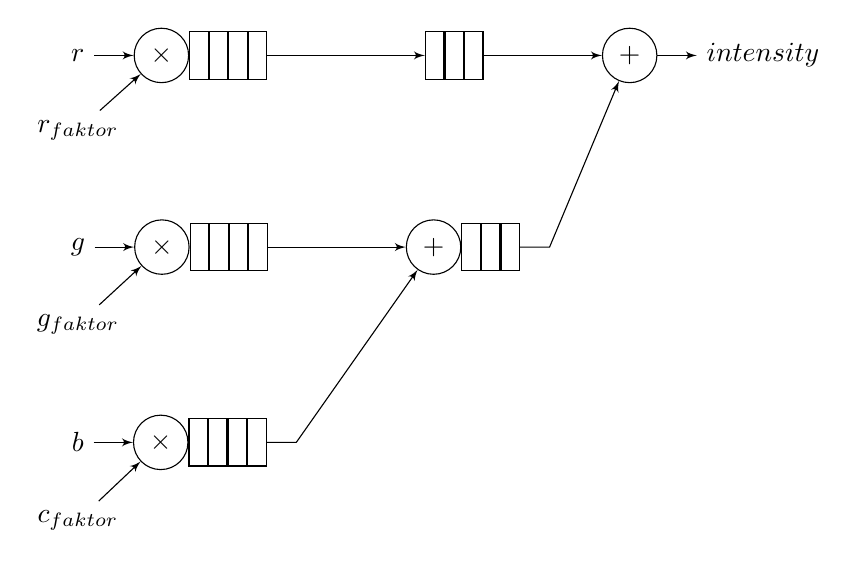
\begin{tikzpicture}[node distance=0.5cm, auto, >=latex']
		\node [] (inr) {$r$};
		\node [below= 0.5cm of inr] (cr) {$r_{faktor}$};
		\node [below= 2cm of inr] (ing) {$g$};
		\node [below= 0.5cm of ing] (cg) {$g_{faktor}$};
		\node [below= 2cm of ing] (inb) {$b$};
		\node [below= 0.5cm of inb] (cb) {$c_{faktor}$};
		\node [draw, circle, right= of inr] (mulr) {$\times$};
		\node [draw, rectangle, right= 0cm of mulr, minimum height=0.6cm] (mulr1) {}; 
		\node [draw, rectangle, right= 0cm of mulr1, minimum height=0.6cm] (mulr2) {};
		\node [draw, rectangle, right= 0cm of mulr2, minimum height=0.6cm] (mulr3) {};
		\node [draw, rectangle, right= 0cm of mulr3, minimum height=0.6cm] (mulr4) {};
		\node [draw, circle, right= of ing] (mulg) {$\times$}; 
		\node [draw, rectangle, right= 0cm of mulg, minimum height=0.6cm] (mulg1) {}; 
		\node [draw, rectangle, right= 0cm of mulg1, minimum height=0.6cm] (mulg2) {};
		\node [draw, rectangle, right= 0cm of mulg2, minimum height=0.6cm] (mulg3) {};
		\node [draw, rectangle, right= 0cm of mulg3, minimum height=0.6cm] (mulg4) {};
		\node [draw, circle, right= of inb] (mulb) {$\times$}; 
		\node [draw, rectangle, right= 0cm of mulb, minimum height=0.6cm] (mulb1) {}; 
		\node [draw, rectangle, right= 0cm of mulb1, minimum height=0.6cm] (mulb2) {};
		\node [draw, rectangle, right= 0cm of mulb2, minimum height=0.6cm] (mulb3) {};
		\node [draw, rectangle, right= 0cm of mulb3, minimum height=0.6cm] (mulb4) {};
		\draw [->] (inr) -- (mulr);
		\draw [->] (cr) -- (mulr);
		\draw [->] (ing) -- (mulg);
		\draw [->] (cg) -- (mulg);
		\draw [->] (inb) -- (mulb);
		\draw [->] (cb) -- (mulb);
		
		\node[draw, circle, right= 2cm of mulg3] (addgb) {$+$};
		\node [draw, rectangle, right= 0cm of addgb, minimum height=0.6cm] (addgb1) {}; 
		\node [draw, rectangle, right= 0cm of addgb1, minimum height=0.6cm] (addgb2) {};
		\node [draw, rectangle, right= 0cm of addgb2, minimum height=0.6cm] (addgb3) {};
		\draw [->] (mulb4) -- ++ (0.5cm,0) -- (addgb);
		\draw [->] (mulg4) -- ++ (0.5cm,0) -- (addgb);
		
		
		\node [draw, rectangle, right= 2cm of mulr4, minimum height=0.6cm] (mulr5) {}; 
		\node [draw, rectangle, right= 0cm of mulr5, minimum height=0.6cm] (mulr6) {};
		\node [draw, rectangle, right= 0cm of mulr6, minimum height=0.6cm] (mulr7) {};
		\draw [->] (mulr4) -- ++ (0.5cm,0) -- (mulr5);
		
		\node[draw, circle, right= 2cm of mulr5] (sum) {$+$};
		
		\draw [->] (mulr7) -- ++ (0.5cm,0) -- (sum);
		\draw [->] (addgb3) -- ++ (0.5cm,0) -- (sum);
		
		\node[right= of sum] (out) {$intensity$};
		\draw [->] (sum) -- (out);
	\end{tikzpicture}
  \caption{RGB to grayscale intensity freeruning conversion pipeline}
\end{figure}


\subsection{Decoupling Processing Stages with Shift Registers}

Shift Registers with intelligent clock enables can be used as an queue that doesn't need counters like a FIFO. I decided to use this kind of decoupling to fulfill adder limitation. For a efficient FIFO implementation with high bandwidth single cycle counters are needed.

\paragraph{Proposed decoupling shift register}
My proposed shift register works in two modes stalled and non stalled. For each data word register there is also a valid register. During non stall cycles elements are inserted at first taken space in the shift register chain and all stored value staring at this place to end are shifted. As opposite during stall cycles elements are added in the first space and all registers until the first invalid registers are shifted forward. The proposed decoupling element preserves sorting because at every time elements are added before the first all ready stored element. During non stall cycles the amount of stored elements stay constant, but free spaces is moved to the front. The amount of elements that can be stored during a stall increases.

\subsection{SLC Implementation}
The SLC implementation is a straight forward conversion of the C version. Because the grayscale conversion can be implemented embarrassingly parallel (map) by assign a micro thread to each pixel to convert. The thread index is used to load the input pixel color and to store after the conversion the intensity value.

\section{Histogram}
The computation of a histogram can be seen as a map reduce operation. Map converts a intensity to a bin index and the reduction counts the occurrence of each index. The map operation is again embarrassingly parallel. 

\subsection{Integer approximation}

The double precision value to bin map functions uses following equation: 

$f(x,b) = round(x*(b-1)/255.0)$

The rounding can be solved be using one bit more precision then needed, therefore the result would be fixed point number with single bit after the decimal point. This bit is one if decimal part is $0.5$ or larger. If this bit is one we easily add one to the integer part. Problematic is the division by $255_{10}=11111111_2$ this can not be implemented with a simple shift. It could be implemented by iterative shifting and subtraction. 

\begin{minipage}{\linewidth}
\begin{lstlisting}[language=C]
static inline uint8_t maptobin(uint8_t p) {
	uint16_t bin = ((uint16_t)p) * (BINS-1);
	bin = (bin >> 8) + ((bin >> 7) & 1);
	return (uint8_t)bin;
}
\end{lstlisting}
\end{minipage}

\subsection{Error Evaluation}

We used in our fix point implementation division by 256 via a simple shift by 8. Because of this difference we assign some values to a lower bin. But for bin values $2^n+1 = {1,2,5,9,17,33,65,129}$ we get exactly the same result.
\begin{figure}[h!]
	\centering
	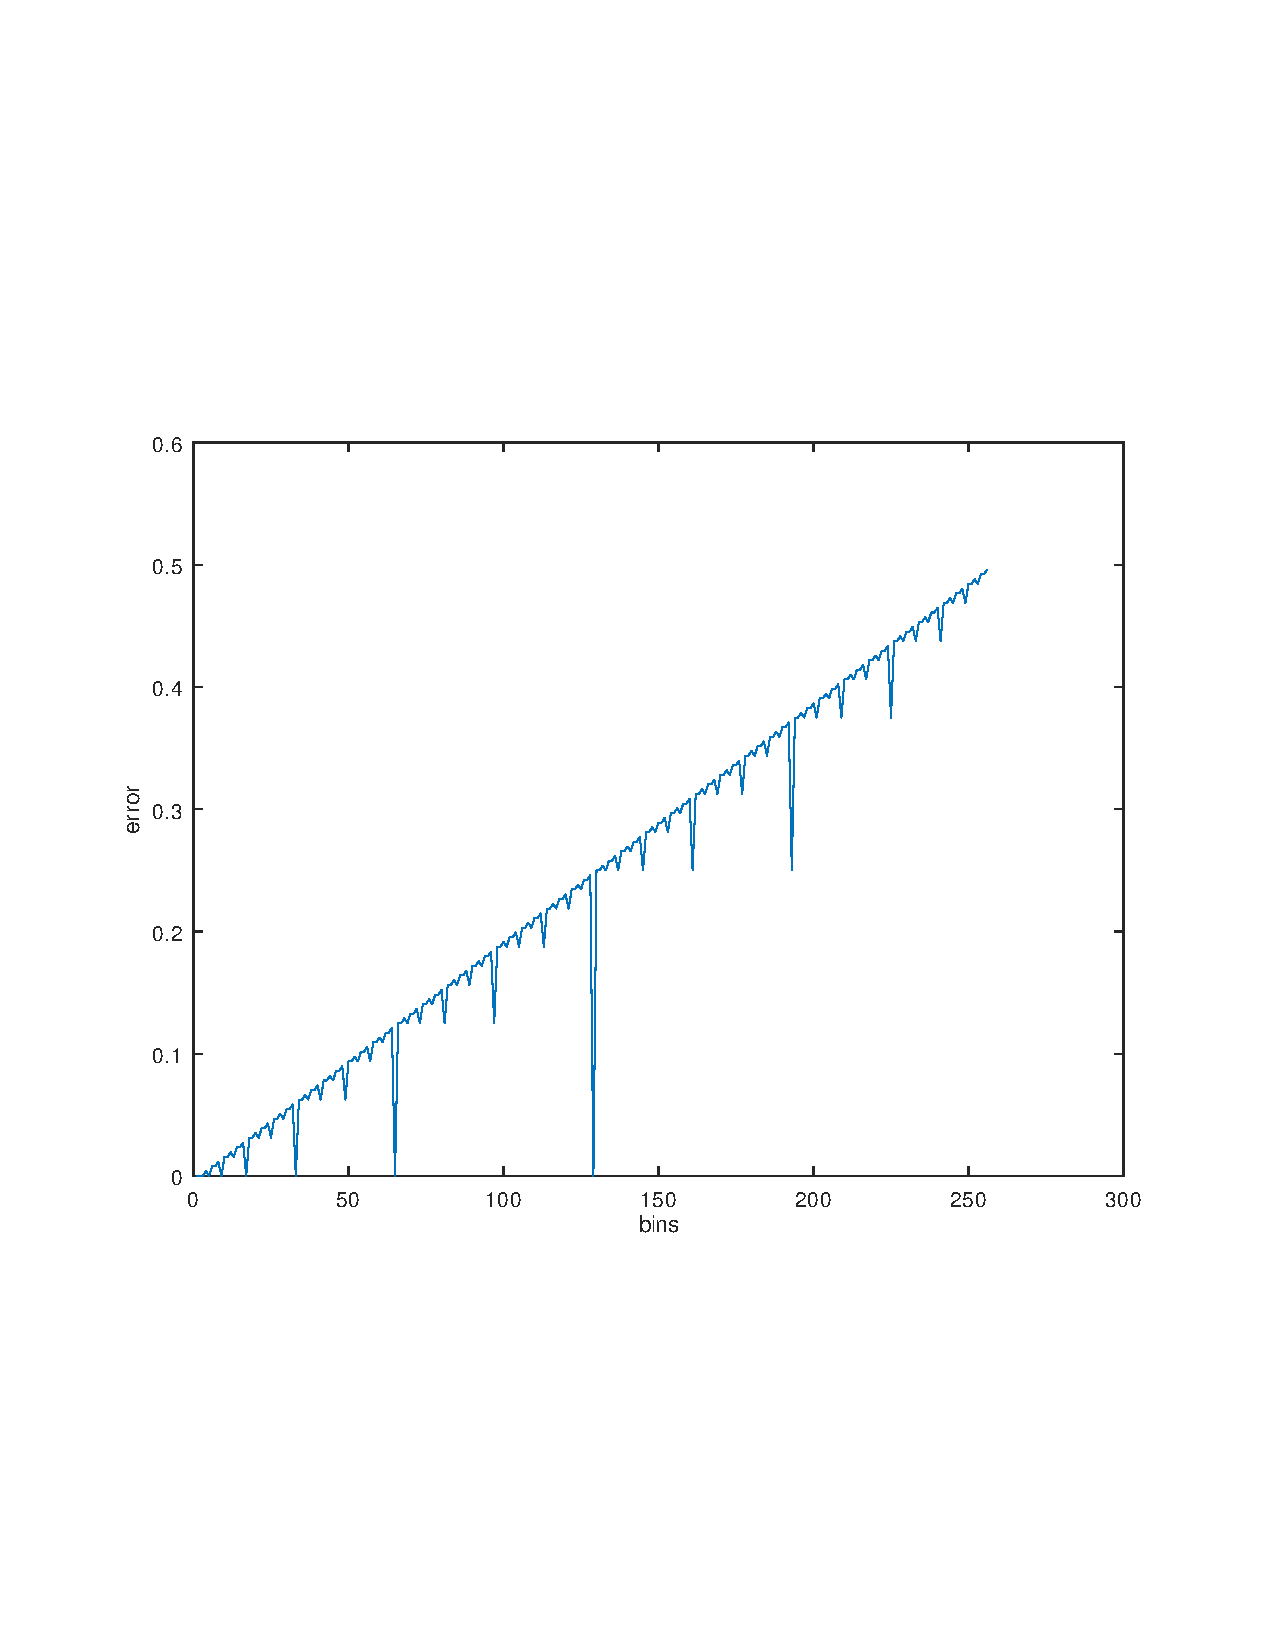
\includegraphics[width=0.4\linewidth]{histoerror}
	\caption{Mean Absolute Error over the 8 Bit value range.}
\end{figure}

\subsection{Datapath}

The datapath for the histogram computation is split in two parts. The map part converting intensity values to bins and the reduction part counting bin occurrence. 

\paragraph{Map}

For the map part i used the same approach as before for the grayscale conversion. A free running pipeline with consecutive shift register decoupler. The pipeline consists of a single multiplier following an adder implementing the rounding. Input for the multiplier is the fixed value $BIN-1$ and the current intensity pixel. Input for the adder is the result of the multiplier shift by 8 and the result shifted by 7 bitwise and 1. This is equivalent to the C implementation. 

\paragraph{Reduce}

The counting of the bin occurrence is done in a Dual Port BRAM, that is extended with a bypass register to solve concurrent read and write of the same address. Without this bypass register the old value would be read and not the new values. Now it is possible to pipeline the counting with the following behavior. Every cycle a incoming bin is read for the BRAM on one port and in every cycle the read value is stored incremented by one. After an reset or start of frame the BRAM must be reseted to zero, for this the incoming data is stalled until all bins are zeroed.


\subsection{SLC Implementation}
To separated the two parts of the histogram computation we are using a communication channel between a parent and succeeding threads. Again we are decomposing the parallel data to a single data point for a single thread. A thread consists of two parts the parallel map from value to bin and the synchronized reduction. For the communication between threads a single shared and dependent register is used through which a pointer to the histogram array is forward. A threads receives the pointer through the shared register. After that the thread reads the bin and stores it incremented and finally forwards the pointer. The section between receiving and forwarding forms a critical section and possible read before write conflicts are solved.

\begin{lstlisting}[language=C]
sl_def(histogram, void, sl_glparm(void*, glInput), sl_glparm(int, glBinMinusOne), sl_shparm(void*, shHistPtr))
{
	sl_index(i);
	uint8_t *in = sl_getp(glInput);
	uint16_t binMinusOne = sl_getp(glBinMinusOne);
	uint16_t binMinusOne = ((uint16_t)in[i]) * (bins);
	bin = (bin >> 8) + ((bin >> 7) & 1);
	
	uint8_t *histo = sl_getp(shHistPtr);
	histo[bin] += 1;
	sl_setp(shHistPtr, histo);
}
sl_enddef
\end{lstlisting}

\section{Sobel-Filter}

\begin{equation*}
G_x = S_x*A = \begin{bmatrix}
1 & 0 & -1 \\
2 & 0 & -2 \\
1 & 0 & -1 \\
\end{bmatrix} * A
\end{equation*}
\begin{equation*}
G_y = S_y*A = \begin{bmatrix}
1 & 2 & 1 \\
0 & 0 & 0 \\
-1 & -2 & -1 \\
\end{bmatrix} * A
\end{equation*}

The Sobel-Operator is a stencil operation that computes gradient images. That can be used to implement an edge dection algorithm. The compute a single output value for the position $(x,y)$ the pixel and its eight neibourghs are neeed.

I propose an offset access function $O((x_1,y_1),((x_2,y_2)) = (x_1+x_2,y_1+y_2)$ that i will used to simplfy the convolutions to a simpler equation. For this i also used follwoing simplfication: $A_{x,y}(P) = A(O((P),(x,y)))$
\begin{equation*}
G_x = A_{-1,-1} + 2 A_{-1,0} +  A_{-1,1} -  A_{1,-1} - 2 A_{1,0} -  A_{1,1}
\end{equation*}
\begin{equation*}
G_y = A_{-1,-1} + 2 A_{0,-1} +  A_{1,-1} -  A_{-1,1} - 2 A_{0,1} -  A_{1,1}
\end{equation*}

\section{C-Implementation}

For the c implementation i used the algorithm described above. The resulting values have a signed range of $[-4\times255, 4\times255]$. To fit the signed back to an 8-Bit unsigned range of $[255,0]$, i shifted the negativ range to $0$ and scaled the range by $8$. Therefor a grandient result of $127_{10}$  means no gradient and results above this value mean a positive gradient and vice versa. The sobel algorith can be implemented without any multiplication by using shifts.

\begin{lstlisting}[language=C]
#define OFFSETACCESS(p, i, j, x, y) (p[(i+x) + (j+y)*HEIGHT])

int main(int argc, const char **argv) {
	int i, j;	
	uint8_t EX[(WIDTH-2)][(HEIGHT-2)];
	uint8_t EY[(WIDTH-2)][(HEIGHT-2)];
	uint8_t ginput[WIDTH*HEIGHT];
	for(i = 0; i < WIDTH*HEIGHT; ++i) {
		ginput[i] = i%2*127;
	}
	
	for(i = 1; i < WIDTH-1; ++i) {
		for(j = 1; j < HEIGHT-1; j++) {
			uint8_t p0 = OFFSETACCESS(ginput, i, j, -1, -1);
			uint8_t p1 = OFFSETACCESS(ginput, i, j,  0, -1);
			uint8_t p2 = OFFSETACCESS(ginput, i, j,  1, -1);
			uint8_t p3 = OFFSETACCESS(ginput, i, j, -1,  0);
			uint8_t p4 = OFFSETACCESS(ginput, i, j,  0,  0);
			uint8_t p5 = OFFSETACCESS(ginput, i, j,  1,  0);
			uint8_t p6 = OFFSETACCESS(ginput, i, j, -1,  1);
			uint8_t p7 = OFFSETACCESS(ginput, i, j,  0,  1);
			uint8_t p8 = OFFSETACCESS(ginput, i, j,  1,  1);
			int16_t ex = (int16_t)p0 - p2 + 2*p3 - 2*p5 + p6 - p8;
			int16_t ey = (int16_t)p0 + 2*p1 + p3 - p6 - 2*p7 - p8;
			ex += 4*255;
			ey += 4*255;
			ex /= 8;
			ey /= 8;
			EX[i-1][j-1] = ex;
			EY[i-1][j-1] = ey;
		}
	}
}
\end{lstlisting}

\subsection{Datapath}

The sobel datapath is split in to two stages. First, i developed a stencil module that transforms the linear stream of pixels to a stream of neighbouring pixel. Second, this stag parallel maps operation are connected converting the neighbouring pixels to the resulting $G_x$ or $G_y$ value.

\paragraph{Conversion from sequetial pixel stream to parallel neighbour stream}

For this i implemented a parameterizable conversion module with the following parameters:
\begin{table}[h]
\begin{tabularx}{\textwidth}{|l|X|}
\hline
\textbf{Parameter} & \textbf{Description} \\ \hline
\hline
C\_ROW\_SIZE & The amount of pixels a single row \\ \hline
p\_dataBits  & The bit width of a single pixel \\ \hline
p\_rows      & The amount of neighborhood row need to compute a single result \\ \hline
p\_cols      & The amount of neighborhood cols need to compute a single result \\ \hline
\end{tabularx}
\end{table}


The conversion is done by using a shift register chain of $(C\_ROW\_SIZE-1)*p\_rows+p\_cols$ registers. The register chain stores pixel data, a valid flag and sof indicator. The first $p\_cols$ registers in each row is connected to the module output. On reset the shift register chain is cleared.

\paragraph{Applying $Gx$ and $Gy$}
For the parallel  compution of $G_x$ and $G_y$ only three adders are used and none multipliers. From this three adders two are combined to a three input adders with total latency of six. Four of the six time categories are used for the two positive and two negative partialsums(State Start\_A to Start\_D).  After that the unwind phase is entered. During unwind the last adder is used to do the value range conversion. This happens during the WAIT\_A and WAIT\_B state. The results are outputted during the DONE state until there are consumed. This module can only consume only one neighborhood vector at a time and is not pipelined and each result computation takes 20 cycles.
\begin{figure}[h]
  \centering
  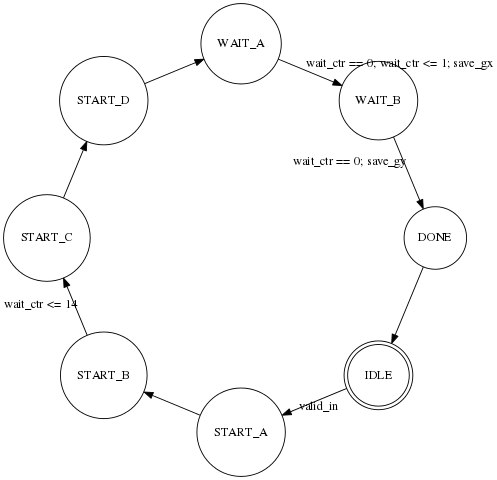
\includegraphics[width=0.5\textwidth]{circofsm.png} 
  \caption{FSM used for computing $G_x$ and $G_y$ with only three adders.}
\end{figure}

\paragraph{Verification}

This datapath is partly written in Verilog and SystemVerilog to improve my SV verfication skills. For verification some edge cases are used and random inputs. As edge cases inputs with all pixel equal are used, these should all result in a $G_x = 127, G_y = 127$ result. All results are evaluated agains a gold standard computed by system verilog.

\pagebreak

\begin{lstlisting}
=================================================================================
=== File: sobel_gx_gy.sv
=================================================================================
    Enabled Coverage            Active      Hits    Misses % Covered
    ----------------            ------      ----    ------ ---------
    Stmts                           64        64         0     100.0
    Branches                        31        29         2      93.5
    FEC Condition Terms              0         0         0     100.0
    FEC Expression Terms             0         0         0     100.0
    FSMs                                                        75.0
        States                       8         8         0     100.0
        Transitions                 22        11        11      50.0
    Toggle Bins                    611       559        52      91.4
\end{lstlisting}

\subsection{SLC Implementation}
The SLC implementation tries to reduce the amount of memory access by forwarding needed values with shared registers. For this approach a family is created for each output row in EX or EX and both outputes are computed at the same time. To compute a single output pixel nine input pixels are needed and to computed the next output pixel in a row six input are overlapping and three new values are needed. Therefore, a single thread is assigned for each output pixel in a row. Each thread need to load threee new values and recevies six values from the previous thread.

\begin{lstlisting}[language=C]
sl_def(sobel, , 
	sl_glparm(void*, a),
	sl_glparm(void*, pex),
	sl_glparm(void*, pey),
	sl_glparm(int, row_length),
	sl_shparm(int, s1), 
	sl_shparm(int, s2),
	sl_shparm(int, s3))
{
	sl_index(i);
	
	const uint8_t *in = sl_getp(a);
	uint8_t (* restrict ex) = (uint8_t *)(void*)sl_getp(pex);
	uint8_t (* restrict ey) = (uint8_t *)(void*)sl_getp(pey);
	uint8_t row_length = sl_getp(row_length);
	
	uint32_t ss1 = sl_getp(s1);
	uint32_t ss2 = sl_getp(s2);
	uint32_t ss3 = sl_getp(s3);
	
	uint8_t p0 = (ss1 & 0xFF);
	uint8_t p1 = (ss1 & 0xFF00) >> 8;
	uint8_t p2 = in[i+2];
	
	uint8_t p3 = (ss2 & 0xFF);
	uint8_t p4 = (ss2 & 0xFF00) >> 8;
	uint8_t p5 = in[i+2+row_length];
	
	uint8_t p6 = (ss3 & 0xFF);
	uint8_t p7 = (ss3 & 0xFF00) >> 8;
	uint8_t p8 = in[i+2+2*row_length];
		
	ss1 = p1 | (p2 << 8);
	ss2 = p4 | (p5 << 8);
	ss3 = p7 | (p8 << 8);
	
	sl_setp(s1, ss1);
	sl_setp(s2, ss2);
	sl_setp(s3, ss3);
		
	int16_t exn = (int16_t)p0 - p2 + 2*p3 - 2*p5 + p6 - p8;
	int16_t eyn = (int16_t)p0 + 2*p1 + p3 - p6 - 2*p7 - p8;

	ex[i] = (uint8_t) ((exn + 4*255)/8);
	ey[i] = (uint8_t) ((eyn + 4*255)/8);
}
sl_enddef
\end{lstlisting}


\appendix
\section{Dynamic Code Traces}
\begin{lstlisting}[language=, caption={Dynamic code trace for grayscale conversion}]
   5742 add
   4416 mov
   3064 ld
   2952 subcc
   2755 ldub
   2378 sll
   2036 and
   2006 st
   1399 nop
   1239 srl
   1200 stb
   858 be
   690 sth
   684 lduh
   675 sra
   675 smul
   662 sub
   652 bleu
   620 ba
   585 std
   479 call
   459 save
   449 restore
   397 clr
   396 bgu
   328 ldd
   301 sethi
   298 or
   258 bl
   254 retl
   224 ret
   220 be,a
   203 bne,a
   200 andcc
   192 bge
   183 bleu,a
   133 bne
   16 clrb
   8 andn
   5 ba,a
   3 jmpl
   3 jmp
   3 ble
   2 ta
   1 sta
   1 flush
   1 bg
   1 bcc
\end{lstlisting}

\pagebreak

\begin{lstlisting}[language=, caption={Dynamic code trace for histogram}]
   7362 add
   6891 mov
   4956 ld
   4883 sll
   3580 and
   3403 subcc
   3264 srl
   3160 st
   2736 nop
   2034 lduh
   1365 sth
   1359 ldub
   975 sethi
   972 or
   929 call
   909 save
   899 restore
   887 sub
   858 be
   735 stb
   710 ble
   704 retl
   606 ba
   585 std
   429 clr
   396 bleu
   396 bgu
   328 ldd
   258 bl
   224 ret
   220 be,a
   203 bne,a
   200 andcc
   192 bge
   183 bleu,a
   133 bne
   8 andn
   5 ba,a
   3 jmpl
   3 jmp
   2 ta
   1 sta
   1 flush
   1 bg
   1 bcc
\end{lstlisting}


\pagebreak

\begin{lstlisting}[language=, caption={Dynamic code trace for sobel filter}]
  11913 mov
  11119 add
  10228 subcc
  9535 ld
  5976 sll
  5555 st
  4614 nop
  4605 be
  4112 and
  3715 srl
  2656 lduh
  2370 sethi
  2341 call
  2327 ldub
  1871 andcc
  1826 save
  1814 restore
  1573 sub
  1510 or
  1464 sth
  1398 ba
  1209 ble
  1203 retl
  1172 stb
  1105 ret
  1094 clr
  1001 bne
  925 be,a
  807 bne,a
  784 sra
  737 bleu
  645 bl
  619 std
  579 bgu
  469 ldsb
  346 ldd
  319 bge
  307 bcc
  277 orcc
  273 bcs
  224 addcc
  216 bg
  183 bleu,a
  181 bl,a
  68 jmp
  62 ldsh
  61 clrb
  61 bge,a
  61 addx
  39 andn
  34 jmpl
  31 ble,a
  31 bg,a
  5 ba,a
  2 ta
  2 rett
  1 sta
  1 flush
\end{lstlisting}

\end{document}